\documentclass{amsbook}

\usepackage[pdftex]{graphicx}
\usepackage{amsmath}
\usepackage{../HBSuerDemir}
\usepackage{wrapfig}

\begin{document}
\par\underline{Equation of the plane through a point and perpendicular} to a vector.
\begin{wrapfigure}{r}{2.5cm}
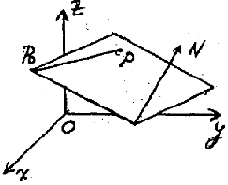
\includegraphics{images/B2P1-163.png}
\end{wrapfigure}
\par Let $P_{0}(x_{0},y_{0},z_{0})$ be the given point and $\overrightarrow{N}$=(A, B, C,) be the vector. Let P(x, y, z) be any point of the plane $\pi$ through P$_{0}$ and perpendicular to $\overrightarrow{N}$. Then\\
$
	\overrightarrow{N}\perp\pi
	\implies\overrightarrow{N}\perp\overrightarrow{P_{0}P}
	\implies\overrightarrow{N}\cdot\overrightarrow{P_{0}P}=0\\
	\overrightarrow{N}\cdot(P-P_{0})=0\quad\big(vector\quad equation
$\\
Then the required equation is
\begin{align*}
	\pi :A(x-x_{0})+B(y-y_{0})+C(z-z_{0})=0\qquad(1)
\end{align*}
or
\begin{align*}
	\pi:Ax+By+Cz+D=0\quad(\underline{general\quad equation})\quad(1')\qquad
\end{align*}
where $D=-Ax_{0}-By_{0}-Cz_{0}$.
\par The vector $\overrightarrow{N}$ is called a \underline{normal vector} or a \underline{direction} vector, and its component A, B, C are direction numbers of the plane $\pi$.
\par Observe taht direction numbers A, B, C appear as coefficients in (1) or in (1'), and hence the planes
\begin{align*}
	Ax+By+Cz+D=0\quad and \quad A'x+B'y+C'z+D'=0
\end{align*}
are parallel if and only if
\begin{align*}
	\frac{A}{A'}=\frac{B}{B'}=\frac{C}{C'}\quad(\overrightarrow{N}\parallel\overrightarrow{N'})
\end{align*}
\par Similarly
\begin{align*}
	AA'+BB'+CC'=0 \iff\pi\perp\pi'
\end{align*}
\par\underline{Remark}. The plane represented by the general equation\\Ax + By + Cz + D = 0 is parallel (perpendicular) to xy-plane when\\A=0, B=0 (C$\neq$). Similar results hold when parallel (perpendicular) to other coordinate planes.
\end{document}